\documentclass[../../Main/Main.tex]{subfiles}

\begin{document}


\chapter{The role of dimension, symmetry and range of interactions in phase transitions}

Which is the role of the dimension in phase transition? Consider \emph{d}, the dimension of the system.
For the Ising model, we have seen that in \( d=1 \) there is no phase transition, while the Onsanger solution tell us that for \( d=2 \) there is a paramagnetic-ferromagnetic transition for \( T_c >0 \).
Therefore, the dimension seems a crucial parameter!
Since in general analytic solutions are not available, is there a simple argument to establish the existence of a phase transition?
In the case of a para-ferro transition, may we establish whether a phase with long range order exists and is stable within a range of \( T>0 \)?

\section{Energy-entropy argument}
We need an argument that can tell us which kind of system has a phase transition. The idea is to use the entropy energy argument. Indeed, our systems are ruled by a free energy and the previous states are found by making derivative. We have energy and entropy: low energy state can be stable with respect to thermal fluctuations, but the fluctuations will destroy the long range order. This idea can be generalized.

Let us consider: 
\begin{equation}
  \dd[]{F} = \underbrace{\dd[]{U}}_{\text{energy}}  - T \underbrace{ \dd[]{S}}_{\text{entropy}}
\end{equation}
We expect that:
\begin{itemize}
\item \( T \gg 1\): entropy should dominates.
\item \( T \ll 1 \): energy should dominates.
\end{itemize}

\noindent Question: there is a temperature different to zero in which this is compatible?

\subsection{\emph{1-dim} Ising}
Let us study the stability of the states with minimum energy to fluctuations for \( T \neq 0 \), for a system of size  \emph{N}.

We already know that, for \( T=0 \), two ground states exist, either all spins up or all spins down.
For instance, suppose that we have the ground state with all the spin up; the energy of the state is
\begin{equation}
   E_G = -JN
\end{equation}
and it is the same for the other configuration.

Now, let us consider \( T \neq 0 \), there could be a given number of elementary excitations of the kind spin up/down. What happens if we swap one or more spins?
These are defects with respect to the ground state and they are also called \emph{domain walls}.
This is in the one dimensional case, but is valid also in many dimensional. Therefore, which is the variation in energy \( \Delta E \) with respect to the ground state?
For each excitation there is an energy penalty \( \Delta E = 2J \), indeed, if we suppose that we have only one swap, we have 
\begin{equation*}
  E_G = -JN, \qquad E^* = -J(N-2) +2J \qquad \Rightarrow \Delta E = 4J
\end{equation*}
For a finite concentration \emph{x} of domain walls, we can write \(   M = Nx \), giving
\begin{equation}
  \Delta E_M = 4MJ
\end{equation}

Now, let us compute the change in entropy.
The entropy of the ground state can be computed immediately: this is zero because it is the logarithm of the number of configurations, but in this case we have only one configuration, namely  \( S_G = \ln{1} =  0 \). Hence, the difference between the entropy of the ground state and the entropy of the new state is just the entropy of the new state.
Therefore, we want to estimate the entropy of the states with \emph{M} domain walls. 
The number of possible ways to insert \emph{M} domains in \emph{N} positions, namely the number of configurations, is
\begin{equation}
  \# = \begin{pmatrix}
  N \\
  M
  \end{pmatrix} = \begin{pmatrix}
  N \\
  xN
  \end{pmatrix}
\end{equation}
We have:
\begin{equation}
  S_M = k_B \log{\begin{pmatrix}
  N \\
  M
  \end{pmatrix}}
\end{equation}
the difference is
\begin{equation*}
  \Delta S = S_M -S_G = S_M = k_B \ln{\begin{pmatrix}
  N \\
  xN
  \end{pmatrix} }
\end{equation*}
Let us calulate
\begin{equation*}
\begin{split}
\Delta F  &= F_M - F_G = \Delta E - T \Delta S  \\
          &= 2 M J - k_B T \ln{\begin{pmatrix}
          N \\
          M
          \end{pmatrix} } \\
          & = 2xNJ - k_B T \ln{\begin{pmatrix}
          N \\
          xN
          \end{pmatrix} } \\
          & = N \qty{ 2xJ +k_B T \qty[x \ln{x} + (1-x)\ln{(1-x)}  ] }
\end{split}
\end{equation*}
where we have used the Stirling approximation
\begin{equation*}
 \ln{N!} = N \ln{N} - N   
\end{equation*}
Since the equilibrium states are obtained by the minimum of \emph{F}, we can minimize with respect to \emph{x}. We are interested in the free energy in the bulk, hence, firstly we normalize and then we derive for finding the minimum
\begin{equation}
  \Delta f_{b_N} = \frac{\Delta F_N}{N}, \qquad \pdv{\Delta f_b}{x} = 0
\end{equation}
this gives 
\begin{equation*}
\begin{split}
  \pdv{}{x} \qty{ 2xJ +k_B T \qty[x \ln{x} + (1-x)\ln{(1-x)}  ] } &=  2J + k_B T \qty[\ln{x} +1 -\ln{(1-x)} -1 ]\\
  & = 2J + k_B T \qty[\ln{x}- \ln{(1-x)}  ] = 0
\end{split}
\end{equation*}
hence,
\begin{equation*}
  \ln{\frac{x}{1-x}} = -\frac{2J}{k_B T} \quad \Rightarrow \frac{x}{1-x} = e^{-2J/k_BT}
\end{equation*}
and finally the results is
\begin{equation}
 x = \frac{1}{1+e^{2J/k_BT} }
 \label{eq:10_3}
\end{equation}
It means that  \( \forall T \neq 0 \) exist a finite concentration \emph{x} of domain walls. The ground state is unstable \( \forall T>0 \). Indeed, if you have a finite density of \emph{x}, no long range order exist for \( T>0 \).  From \eqref{eq:10_3}, we can see that as \( T \rightarrow 0 \),  we have \( x \rightarrow 0\) as expected.
So there are \textbf{no ordered phases} $\forall \, T > 0$.
Now, let us try to do the same for \emph{d} dimensions.

\subsection{\emph{d-dim} Ising}
What is a \emph{domain wall} in \emph{d} dimensions? The domain walls is an hypersurface of size \( L^{d-1} \)
\begin{equation}
  \Delta E \propto 2JL^{d-1}
\end{equation}
Computing the entropy it is a very difficult problem. Indeed, the entropy of a fluctuating hypersurface is difficult to estimate. 
For a single domain wall, we can say
\begin{equation}
  S \propto k_B \ln{\mu^L} = k_B L \ln{\mu}
\end{equation}
where  \( \mu^{\emph{L}} \) is the number of ways to place a straight wall within a system of linear size \emph{L}.
The \( \Delta S \)  is just \emph{S}  because the entropy of the ground state is again zero.
\begin{remark}
If we underestimate \emph{S}, we obtain
\begin{equation}
  \Delta F = 2JL^{d-1}-k_B T L \ln{\mu}
\end{equation}
it means that now energy can win if the temperature is different from zero. Therefore, for \( d=2 \),  or greater (\( d>1 \)), that long range order can survive  thermal fluctuations and the system could present an ordered phase!
\end{remark}

\subsubsection{$d = 2$ with fixed boundary conditions}

\begin{figure}[h!]
\centering
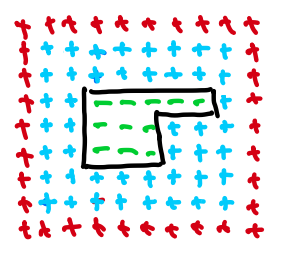
\includegraphics[width=0.5\textwidth]{./img/IMG1.png}
\caption{\label{fig:10_1} System with boundary condition with all the spins in the surface up.}
\end{figure}


The domain wall is a bubble of down spins in a ground state of "up" spins. The polygon is of length $L$ and the energy difference is $\Delta E = E_{L} - E_{G} = 2LJ$. The number of polygons of length $L$ with fixed origin is $\approx \mu^{L}$ with $2 < \mu < 3$. Since the origin can be moved in $N$ sites then $S_{L} \approx k_{b}\ln[N \mu^{L}]$ and
$$\Delta f < 0 \Leftrightarrow L \leq \frac{k_{B}T\ln N}{2J - k_{B}T\ln \mu}$$
So for $T < \frac{2J}{k_{b}\ln \mu}$ the bubbles have a small probability for $L \geq L_{max}$. The $\%$ of down spins is $\sim \frac{L^{2}}{N} \sim \frac{(\ln N)^{2}}{N} \to 0$. So $m \neq 0$ is possible if $T \leq \frac{2J}{k_{B}\ln \mu}$.




\subsubsection*{Peierls argument}
The Peierls argument \cite{10_lesson_1} is a mathematically rigorous and intuitive method to show the presence of a non-vanishing spontaneous magnetization in some lattice models. This argument is typically explained for the \(d=2\) Ising model in a way which cannot be easily generalized to higher dimension.
The idea is trying to perturb the system using an external magnetic field as perturbation (it is very small \emph{h}). In that way, we are breaking explicitly the symmetry, but then, taking the limit \( h \rightarrow 0 \) and switching off the magnetic field, we see the stability.

 We know that for finite systems, from the \( \mathbb{Z}^2 \) symmetry, it follows
\begin{equation*}
  \expval{m}_N = 0
\end{equation*}
This is true for finite systems, however, in the thermodynamical limit \( N \rightarrow \infty  \), if \(d \ge 2\) the magnetization \( \expval{m}_{\infty } \) vanishes only in the high temperature paramagnetic phase. 
In the low temperature ferromagnetic phase, the value of \( \expval{m}_{\infty } \) is not well defined and depends on how the thermodynamical limit is performed. In this case the \( \mathbb{Z}^2\) symmetry  is said to be spontaneously broken.

The breaking of a symmetry can be thought as a form of thermodynamical instability: the particular value acquired by \( \expval{m}_{\infty } \) in the ferromagnetic phase is determined by small perturbations.

A conventional way to uniquely define \( \expval{m}_{\infty } \) in the broken phase (where it is called spontaneous magnetization) is to use an infinitesimal magnetic field:
\begin{equation}
  \expval{m}_{\infty } = \lim_{h \rightarrow 0^+} \lim_{N \rightarrow \infty } \expval{m}_N^{(h)}
\end{equation}
where it is crucial to perform the thermodynamical limit before switching off the magnetic field \( h \rightarrow 0^+ \). The instability manifests itself in that using \( h \rightarrow 0^- \)  would change the sign of \( \expval{m}_{\infty } \).

A different approach to expose the instability is the use of appropriate boundary conditions:
we can for example, if we want \( \expval{m}_ \infty  > 0\), impose in all the sites \(i\) on the lattice boundary (\( i \in \partial{\Omega }  \)) the condition
\( S_i = +1 \),  as in Figure \ref{fig:10_1}.

\begin{figure}[h!]
\centering
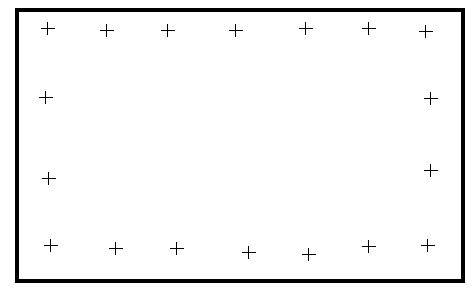
\includegraphics[width=0.5\textwidth]{./img/1.pdf}
\caption{\label{fig:10_1} System with boundary condition with all the spins in the surface up.}
\end{figure}

In the paramagnetic phase the effect of boundary conditions does not survive the thermodynamical limit, while in the ferromagnetic phase their effect is analogous to that of the infinitesimal magnetic field.
%\begin{remark}
 %It is equivalent, because on the border we have a very high field, but it is at the border, so it do not really count for the surface internal. This is a very smart way to do this perturbation of the surface. This particular configuration with all the spin up will give us a particular shape. We can do this also in higher dimensional and we can also estimate the temperature.
%\end{remark}

This is the boundary condition chosen by Pierls to establish the existence of a \( T_c \neq 0 \) for the \(d=2\) Ising model.
Let us gives just a qualitative presentation  of the (rigorous) result. 

Let \( N_+,N_- \) be the number of spin up and down respectively. Clearly,
\begin{equation*}
  N=N_+ + N_-  
\end{equation*}
On a finite lattice the mean value of the magnetization can be written in the form 
\begin{equation*}
  \expval{m}_N = \frac{\expval{N_+} - \expval{N_-}  }{N} = 1 - 2 \frac{\expval{N_-} }{N}
\end{equation*}
In order to show that \( \expval{m}_ \infty >0  \) (remember that we are considering boundary conditions with spin up at \( \partial{\Omega }  \)), it is sufficient to show that for every \(N\) we have 
\begin{equation}
  \frac{\expval{N_-} }{N}  < \frac{1}{2}- \varepsilon
  \label{eq:10_1}
\end{equation}
with \( \varepsilon >0 \) and \(N\)-independent.
Indeed, if \eqref{eq:10_1} holds
\begin{equation}
  \expval{m}_N \ge 2 \varepsilon \quad \forall N
\end{equation}
The Peierls argument is a simple geometrical construction that can be used to prove this
bound.
The outcome of the Peierls argument for the model in \(d\) dimensions is an estimate of the form
\begin{equation}
  \frac{\expval{N_-} }{N} \le f_D (x)
\end{equation}
where \(x\) is defined by 
\begin{equation}
  x = 9 e^{-4J \beta } 
\end{equation}
and \( f_D \) is a continuous function of \( x \) (independent on \emph{N}) and such that 
\begin{equation*}
\lim_{x \rightarrow 0} f_D (x) = 0    
\end{equation*}
In particular, for small enough \emph{T} we have the bound
\begin{equation*}
  \frac{\expval{N_-} }{N} < \frac{1}{2} - \varepsilon
\end{equation*}
which ensures that \(\expval{m}_\infty \ge 2\varepsilon  \) and the \(\mathbb{Z}^2\) symmetry is spontaneously broken.
More precisely, for \(d=2\), one has
\begin{equation}
    \frac{\expval{N_-} }{N} \le \frac{x^2}{36} \frac{2-x}{(1-x)^2}
\end{equation}
where \(   x = 9 e^{-4J \beta } < 1 \).

\begin{remark}
Note that above bound gives also a lower bound on the critical temperature
\begin{equation*}
    \frac{\expval{N_-} }{N} \le \frac{x^2}{36} \frac{2-x}{(1-x)^2} < \frac{1}{2} - \varepsilon
\end{equation*}
As long as \(   \frac{\expval{N_-} }{N}  < \frac{1}{2} - \varepsilon  \), the system is in the ferromagnetic phase. The critical value \( x_c \equiv x (\beta _c) \) must be outside the interval \( [0,x_{1/2}] \) where \( x_{1/2} \)   is the smallest positive solution of the equation
\begin{equation*}
  \frac{x^2}{36} \frac{2-x}{(1-x)^2} = \frac{1}{2}
\end{equation*}
From the solution \( x_{1/2} \) and the condition \( x_c > x_{1/2} \), one has
\begin{equation*}
  J \beta _c \le J \beta_{1/2}
\end{equation*}
where \( J \beta _{1/2} = \frac{1}{4} \log{9/x_{1/2}}  \). 
Hence, \( T_c > T_{1/2} \).
\end{remark}

\begin{exercise}{}{}
The following equation gives \( x_{1/2} \):
\begin{equation*}
  x^3 + 16x^2 - 36 x + 18 = 0
\end{equation*}
 Find \( T_{1/2} \).
\begin{solution}
This equation has three real solutions:
\begin{equation*}
    x_1 =-18.05, \quad x_2=0.79, \quad x_3=1.26
\end{equation*}
The smallest positive solutions is \( x_{1/2} \equiv x_2 \), hence 
\begin{equation*}
\frac{J}{k_B T_{1/2} } = \frac{1}{4} \log{9/x_{1/2}} \quad \Rightarrow 
T_{1/2} = \frac{4J}{k_B \log{9/x_{1/2}}}
\end{equation*}
\end{solution}
\end{exercise}


\clearpage
\section{Role of the symmetry}
Interacting systems can be classified with respect to their \emph{global symmetry group}. Let us illustrate some examples.
\begin{example}{Ising model}{}
  \begin{equation}
    \mathcal{H}_{\text{Ising}} = - \sum_{i<j}^{} J_{ij} \sigma _i \sigma _j
  \end{equation}
  where \( \sigma _i \in \{ -1,1 \}   \). The symmetry group of this Hamiltonian is \( \mathbb{Z}^2 \), which has two elements \( \{ \mathbb{1}, \eta  \}   \). We have
  \begin{equation*}
    \mathbb{1}: \text{ identity}, \quad \eta \sigma _i = - \sigma _i, \quad \eta ^2 = \mathbb{1}
  \end{equation*}
\end{example}
\begin{example}{Potts model}{}
The Potts model, a generalization of the Ising model, is a model of interacting spins on a crystalline lattice. The Hamiltonian is 
  \begin{equation}
    \mathcal{H}_{q- \text{Potts}} = - \sum_{i<j}^{} J_{ij} \delta _{\sigma _i, \sigma _j}
  \end{equation}
  where \( \sigma _i \in [1,2,3,\dots,q] \). \( \mathcal{H}_{q- \text{Potts}} \)  is invariant under the permutation group of the sequence \( \{ 1,2,3,\dots,q \}   \). There are \( q! \) elements, for example \( \{ 2,1,3,\dots,q \}   \). The symmetry group is denoted by \( S_q \).
\end{example}
\begin{remark}
The difference between a \( \mathbb{Z}_q \) and \( S_q \) symmetry is that an Hamiltonian has symmetry \( \mathbb{Z}_q \) if it is invariant with respect to \emph{cyclic permutations}\footnote{In mathematics, and in particular in group theory, a cyclic permutation (or cycle) is a permutation of the elements of some set \(X\) which maps the elements of some subset \(S\) of \(X\) to each other in a cyclic fashion, while fixing (that is, mapping to themselves) all other elements of\(X\). If \(S\) has \(k\) elements, the cycle is called a \(k\)-cycle. Cycles are often denoted by the list of their elements enclosed with parentheses, in the order to which they are permuted.}
\begin{equation}
  \eta = \begin{pmatrix}
    1 & 2 & \dots & q-1 & q \\
    2 & 3 & \dots & q & 1
  \end{pmatrix}
\end{equation}
and its powers \( \eta ^l \) with \( l=0, \dots, q-1 \). Both models satisfy a \emph{discrete global symmetry}.
\end{remark}
Now, we jump into the case in which we consider \emph{continuous} symmetries.


\begin{figure}[h!]
\centering
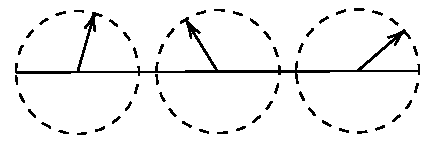
\includegraphics[width=0.5\textwidth]{./img/2.pdf}
\caption{\label{fig:10_2} Spin can assume all values around the circles.}
\end{figure}

\begin{example}{XY model}{}


This is a spin model that is invariant with respect to the continuous global symmetry
\( \theta _i \rightarrow \theta _i + \alpha  \).
Indeed, the Hamiltonian of this model is
\begin{equation}
  \mathcal{H}_{XY} = - \sum_{i<j}^{} J_{ij} \va{S}_i \vdot \va{S}_j
\end{equation}
where \(\va{S}_i  \) is a \( 2D \) spin vector
\begin{equation*}
  \va{S}_i = (S_{x_i}, S_{y_i})
\end{equation*}
that can assume values on the unit circle ( \(  \abs{\va{S}_i} =1 \)).
Suppose that spins are sitting in hyper dimensional and can rotate along circles. They can assume all the value as in Figure \ref{fig:10_2}.

The simplest way to parametrize the Hamiltonian is by the angle.
Denoting by \( \theta _i \) the direction angle of spins \( \va{S}_i \), the Hamiltonian can be rewritten as
\begin{equation}
  \mathcal{H}_{XY} = - \sum_{i<j}^{} J_{ij} \cos(\theta _i - \theta _j)
\end{equation}
with \( \theta _i \in [0,2 \pi ] \).

\begin{remark}
The interaction term \( \cos(\theta _i - \theta _j)  \) can be written also as
\begin{equation*}
  \frac{1}{2} \qty(Z_i^* Z_j + Z_i Z_j^*)
\end{equation*}
where \(   Z_j = \exp (i \theta _j) \).
\end{remark}

The model is invariant under the global transformation
\begin{equation}
  Z_i \rightarrow e^{i \alpha } Z_i
\end{equation}
The phase  \( \exp (i \alpha )  \) form a group under multiplication known as \( U(1) \) that is equivalent to \( O(2) \). Indeed, the interaction term can be written also as
\begin{equation*}
  \vu{\Omega }_i \vdot \vu{\Omega }_j
\end{equation*}
where \( \vu{\Omega }_i = ( \cos \theta _i, \sin \theta _i) \).
\begin{remark}
In \emph{n}-dimensions \( \vu{\Omega } \) has \emph{n} components  \( \vu{\Omega } = \{ \Omega ^1, \Omega ^2, \dots, \Omega ^n \}   \)  and the corresponding Hamiltonian is
\begin{equation}
  \mathcal{H} = - \sum_{i>j}^{} J_{ij} \vu{\Omega }_i \vdot  \vu{\Omega }_j
\end{equation}
It is symmetric with respect to the global symmetry group \( O(n) \).
\end{remark}
\end{example}

 Which are the domain walls for continuous symmetries? Which are the implications for the stability of the ordered phase?

\section{Continuous symmetries and phase transitions}
\subsection{XY model with n.n. interactions}
$$\mathcal{H}_{XY} = - \sum_{\avg{{ij}}} J_{ij} \cos(\theta_{i}- \theta_{j})$$
With the $\theta_{i}$ the angle between the horizontal and the spin so $\theta_{i} \in [-\pi,\pi]$ of spin $\hat{s}_{i}$ and $\mid \hat{s}_{i}\mid = 1$.
The partition function for $N = L^{d}$ spins and $H = 0$ is
$$Z_{N}(T,J) = \int_{-\pi}^{\pi} \prod_{k=1}^{N}\exp\left( \beta J \sum_{\avg{ij}} \cos(\theta_{i}-\theta_{j})\right) \, d\theta_{k} $$

Note that if we consider a chain of spins $d = 1$ then $Z_{N}(T,J)$ can be computed exactly for either \textbf{free boundary conditions} using the method used for the Ising and suggested for Heinsenberg or \textbf{periodic boundary conditions (ring of spins)} with the transfer matrix method.
Since here we are interested in the stability of ordered (ground) state we can look at the \textbfz{low temperature approximation}.




\subsection{Low Temperature approximation of the n.n. XY model}

If $T \ll 1$ then $\beta \gg 1$ and the most probable configurations are those where $\cos \mid \theta_{i} - \theta_{j}\mid \approx 1$ so where $\mid \theta_{i} - \theta_{j}\mid \ll 1$, the so-called \textbf{Small Deviations}.

This approximation is also known as the \textbf{Gaussian Approximation} since 
$$Z_{N}(T,J) \approx \underbrace{ \int _{-\pi}^{\pi} \prod_{k=1}^{N}\exp\left( \beta J \sum_{\avg{ij} }\left( 1 - \frac{(\theta_{i} - \theta_{j})^{2}}{2} \right) \right) \, d\theta_{k} }_{ \propto \text{ Gaussian Integral} } $$

Note that the term $\mid \theta_{i} - \theta_{j}\mid$ can be seen as the \textit{Finite Difference Approximation} of the operator along the $i \to j$ direction, namely
$$\sum_{\avg{ij} } \frac{1}{2}(\theta_{i} - \theta_{j})^{2} = \sum_{i} \sum_{j \in nn(i)} \frac{(\theta_{i} - \theta_{j})^{2}}{2} \approx \sum_{i} \frac{\nabla \theta}{2} \approx \int \frac{(\nabla \theta(\vec{r}))^{2}}{2} \, d\vec{r} $$
So the Hamiltonian can be written as:
\begin{equation}
  \mathcal{H} = E_0 + \underbrace{\frac{J}{2} \int_{}^{} \dd[]{\va{r}} \qty(\grad \theta )^2 }_{E \equiv \text{Stifness energy}}
\end{equation}
where \( E_0 = JN \) is the energy corresponding to the case in which all the spins are oriented along a given direction. $\Delta E$ is defined as
  \begin{equation}
    \Delta E = \frac{J}{2} \int_{}^{} \dd[]{\va{r}} \qty(\grad \theta )^2
  \end{equation}

\subsubsection{Domain Walls at $T << 1$, continuous symmetry}

When the symmetry is continuous, as for the XY model, good domains are those that smoothly interpolate between opposite ordered regions
\begin{figure}[h!]
\centering
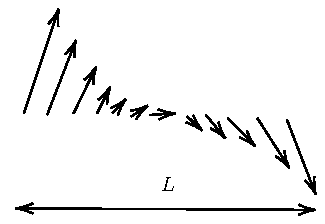
\includegraphics[width=0.4\textwidth]{./img/3.pdf}
\caption{\label{fig:10_3} For continuous symmetry the domain walls interpolate smoothly between two ordered regions.}
\end{figure}
Let us now estimate the energy cost $\Delta E$ to create such state starting from one of the infinite set of ground state that we can pickup using a specific boundary condition.

How it is compose to systems with Ising $\mathbb{Z}^{2}$ symmetry where $\Delta E \propto 2JL^{D-1}$? Since we are close to the ground state then $T \ll 1$ and we can use the
\subsubsection{Spin Stiffness Energy}
  \begin{equation}
    \Delta E = \frac{J}{2} \int_{}^{} \dd[]{\va{r}} \qty(\grad \theta )^2
  \end{equation}
Where $\theta(r)$ is the angle of local rotation around and axis and $J$ is the Spin Rigidity. For and ordered phase $\theta(r) = \theta_0$ and $\mathcal{H}(\mathbf{E}) = E_{0}$

Let us now imagine a domain wall where \(\theta (\va{r})  \)  rotates by \( 2 \pi  \) (or \( 2 \pi m \)) by using the entire length of the system (see again Figure \ref{fig:10_3}):
\begin{equation*}
  \theta (\va{r}) = \frac{2 \pi n x}{L}
\end{equation*}
where \emph{n} is the total number of \( 2 \pi  \) turn of \( \theta  \) in \emph{L}. 
\begin{remark}
Note that there is no variation along the other \( d-1 \) dimensions, therefore we just doing over one dimension.
\end{remark}

We consider only the term \emph{E} (Stifness energy) of the Hamiltonian 
 \begin{equation}
   E = \frac{J}{2} L^{d-1} \int_{0}^{L} \dd[]{x} \qty(\dv{}{x} \qty(\frac{2 \pi n x}{L})  )^2 = \frac{J}{2} L^{d-1} \int_{0}^{L} \dd[]{x} \qty(\frac{2 \pi n}{L})^2 = 2 \pi ^2 n^2 J L^{d-2}
 \end{equation}
\begin{remark}
Unlike the Ising model where \( E \sim L^{d-1} \), here \( E \sim L^{d-2} \)! Hence, if \( S \ge k_B \ln{L}  \) for a single domain wall, \emph{S} should dominate if \( d \le 2 \), the ordered phase is always unstable and no phase transition is expected for \( T \neq 0 \)!
\end{remark}

\begin{definition}{Lower critical dimension}{}
  The Lower Critical dimension \( d_c \) is the dimension at which (and below which) the system does not display a ordered phase (there is no long range order).
  In other words if \( d \le d_c \), we have \( T_c = 0 \).
\end{definition}
 From what we have found before we can say that
\begin{itemize}
\item For discrete global symmetries: \( d_c =1 \).
\item For continuous global symmetries: \( d_c =2 \) (Merming-Wagner theorem)\footnote{In statistical mechanics, the Mermin–Wagner theorem states that continuous symmetries cannot be spontaneously broken at finite temperature in systems with sufficiently short-range interactions in dimensions \(d \le 2\). Intuitively, this means that long-range fluctuations can be created with little energy cost and since they increase the entropy they are favored.}.
\end{itemize}

\begin{example}{\(\pmb{XY}\) model transition}{}
The \(XY\) model in \( d=2 \) is rather special. While the Mermin–Wagner theorem prevents any spontaneous symmetry breaking on a global scale, ordering transitions of Kosterlitz-Thouless-type may be allowed.
 This is the case for the \(XY\) model where the continuous (internal) \( O(2) \) symmetry on a spatial lattice of dimension \(d \le 2\),  remains zero for any finite temperature \( T \neq 0 \) (it do not display an ordered phase).
\begin{remark}
This transition does not imply the spontaneous breaking of the \( O(2) \) symmetry!
\end{remark} 
However, the theorem does not prevent the existence of a phase transition in the sense of a diverging correlation length \(\xi\). To this end, the model has two phases: 
\begin{itemize}
    \item a conventional disordered phase at high temperature with dominating exponential decay of the correlation function 
\(G(r)\sim \exp(-r/\xi )\) for \(r/\xi \gg 1\);
\item a low-temperature phase with quasi-long-range order where \(G(r)\) decays according to some power law, which depends on the temperature, for "sufficiently large", but finite distance \(r\) (\(a \ll r \ll \xi\) with \(a\) the lattice spacing).
\end{itemize}

The transition from the high-temperature disordered phase with the exponential correlation to this low-temperature quasi-ordered phase is a Kosterlitz–Thouless transition. It is a phase transition of infinite order.

In the \(d=2\) XY model, vortices are topologically stable configurations. It is found that the high-temperature disordered phase with exponential correlation decay is a result of the formation of vortices. Vortex generation becomes thermodynamically favorable at the critical temperature \(T_{KT}\) of the KT transition. At temperatures below this, vortex generation has a power law correlation (hence, there is no long range order for \( T<T_{KT} \)).

Many systems with KT transitions involve the dissociation of bound anti-parallel vortex pairs, called vortex–antivortex pairs, into unbound vortices rather than vortex generation. In these systems, thermal generation of vortices produces an even number of vortices of opposite sign. Bound vortex–antivortex pairs have lower energies than free vortices, but have lower entropy as well.

In order to minimize free energy, \(F=E-TS\), the system undergoes a transition at a critical temperature, \(T_{KT}\).
Below \(T_{KT}\) there are only bound vortex–antivortex pairs. Above \(T_{KT}\), there are free vortices.
\end{example}
\subsection{Vortices}

At low temperatures, in addition to the long-wave length \textbf{Spin Waves} (longitudinal fluctuations), there is another class of fluctuations (transverse fluctuations).

To see this let us compute the profiles $\theta(\vec{r})$ corresponding to local minima of $\mathcal{H}$. These are the solutions of the functional differential eq.
$$\begin{aligned}
\frac{\delta \partial}{\delta \theta\left(\vec{r}^{\prime}\right)} & =0, \quad H=\int|\nabla \theta|^2 d r   \Leftrightarrow \nabla^2 \theta\left(\vec{r}^{\prime}\right)=0 .
\end{aligned}$$
The first set of solution: $\theta\left(\bar{r}^{\prime}\right)=$ constant (ground state).
The second set are \texbf{Vortices}. They are obtained by imposing the following set of conditions:

\begin{enumerate}[label=(\alph*)]
    \item $\forall$ closed curves $\Gamma$ enclosing the position $\vec{r}_0$ of the centre of the vortex topological charge $$\oint_{\Gamma} \bar{\nabla} \theta\left(\vec{r}^{\prime}\right) \cdot d \vec{r}^{\prime}=2 \pi n$$
    \item If $\Gamma$ does not include $\vec{r}_{0}$ $$\int _{\Gamma}\nabla \theta(\vec{r}) \, d\vec{r} = 0$$
\end{enumerate}

\begin{figure}[h!]
\centering
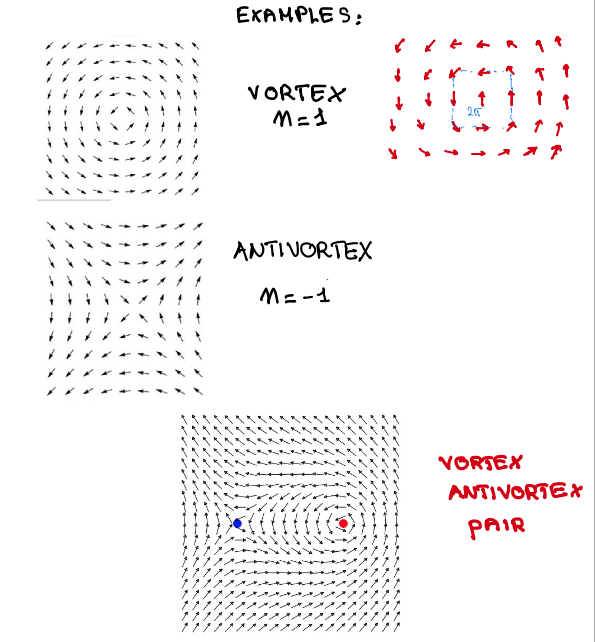
\includegraphics[width=0.5\textwidth]{./img/IMG2.png}
\end{figure}


\subsubsection{Energy Cost of creating a vortex out of a ground state}

Spherical symmetry $\Rightarrow \theta_{\text {vor}}\left(\bar{r}^{\prime}\right)=\theta_{\text {vor}}(r)$
From the definition of topological charge
$$\begin{aligned}
& \Rightarrow 2 \pi n=\oint_{\Gamma} \nabla \theta\left(\vec{r}^{\prime}\right) \cdot d \vec{r}^{\prime}=2 \pi r|\nabla \theta| \\
& \Rightarrow|\nabla \theta|=\frac{n}{r}
\end{aligned}$$
on the other hand we have the spin stiffness energy:
$$\begin{aligned}
& \Rightarrow E_{vor}-E_0=\frac{J}{2} \int d \vec{r}|\vec{\nabla} \theta|^2 \\
& =\frac{J n^2}{2} \int_0^{2 \pi} \int_a^L r d r \frac{1}{r^2} \\
& =\pi n^2 J \ln \left( \frac{L}{a} \right) \\
&
\end{aligned}$$
Where $a$ is the core size, $L$ is the linear size of the $2D$ lattice. Notice that there is a logarithmic divergence.

\subsubsection{Free Energy Argument for a $n = 1$ vortex}
$$\Delta E_{\text {1vortex }}=\pi J \ln \left( \frac{L}{a} \right)$$
To compute the entropy $\Delta S=S_{1 \text {vortex}}$ (the ground state has entropy zero) we can assume that the vortex can be placed in $(I / a)^2$ ways $(D=2)$
$$\begin{aligned}
& \Rightarrow \Delta S=K_b \ln \left[(I / a)^2\right] \\
& \Delta F=\left(\pi J-2 K_b J\right) \ln [L / a]
\end{aligned}$$
We can then reduce the free energy by adding a vortex to a vortex free system as long as $\pi J-2 K_b T<0$
$$\Leftrightarrow \quad T>\frac{\pi}{2} \frac{J}{K_b} \equiv T_{K T} \quad \begin{aligned}
& \text { Kosterlitz } \\
& \text { Thoules } \\
& \text { Temperature }
\end{aligned}$$

The full problem requires the notion of  the vortex-antivortex unbindg mechanism.






\section{Role of the interaction range}
So far we have considered models where the interactions were short range. How things change if long range are considered instead? How does the symmetry broken depends on the range of interactions?

One can show, for example, that if
\begin{equation}
  J_{ij} = \frac{J}{\abs{\va{r}_i - \va{r}_j}^\alpha  }, \quad 1 \le \alpha \le 2
\end{equation}
phase with long range order is stable for \( 0 < T < T_c \) also for \( d=1 \)!  

\begin{remark}
If \( \alpha > 2 + \varepsilon  \) we get back the physics found for short range interactions. If \( \alpha <1 \) the thermodynamic limit does not exist.
\end{remark}

A limiting case of long range interaction is the \emph{infinite range} case where all the spins interact one to another with the same intensity independently on their distance. No metric is involved (instead of previously where the definition of \emph{J} of before is a metric.). It can be solve exactly and later we will see why.

\subsection{Ising model with infinite range}

Let us consider the Hamiltonian 
\begin{equation}
  -\mathcal{H}_N (\{ S \} ) = \frac{J_0}{2} \sum_{i,j}^{N} S_i S_j + H \sum_{i}^{}  S_i
\end{equation}
with \( S_i \in [-1,+1] \).
\begin{remark}
The sum over \(i,j\) is an unrestricted double sum.
\end{remark}
The problem with the double sum is that
\begin{equation*}
  \sum_{i,j}^{} S_i S_j \propto O(N^2)
\end{equation*}
and the thermodynamic limit is ill-defined. To circumvent this problem Mark Kac suggested to consider a strength
\begin{equation}
  J_0 = \frac{J}{N}
\end{equation}
this is called the \emph{kac approximation}. 
Hence,
\begin{equation}
  -\mathcal{H}_N (\{ S \} ) = \frac{J}{2N} \sum_{i,j}^{N} S_i S_j + H \sum_{i}^{}  S_i
\end{equation}
with this choice we recover \( E \sim O(N) \).  

%In this Hamiltonian since you have no metric you have no dimension.













The partition function is

\begin{equation}
Z_N (T,J,H) = \sum_{\{ S \}  }^{} \exp [\frac{\beta J}{2N} \sum_{ij}^{} S_i S_j + \beta H \sum_{i}^{} S_i    ]
\end{equation}
Since there are no restrictions on the double sum, we can write
\begin{equation*}
  \sum_{ij}^{} S_i S_j  = \qty(\sum_{i}^{} S_i ) \qty(\sum_{j}^{} S_j )= \qty( \sum_{i}^{} S_i )^2
\end{equation*}
Rewriting the partition function, we have:
\begin{equation}
  Z_N (T,J,H)  =   \sum_{\{ S \}  }^{} \exp  [\frac{K}{2N} \qty( \sum_{i}^{} S_i )^2 + h \sum_{i}^{} S_i    ]
\end{equation}
\begin{remark}
Recall that we have defined \(K=\beta J\) and \( h = \beta H\).
\end{remark}

In order to transform the quadratic term into a linear one we make use of the integral identity known as the \emph{Hubbard–Stratonovich transformation} (we can do it in any dimension). 
Let 
\begin{equation*}
 x \equiv \sum_{i}^{} S_i
\end{equation*}
The key identity in the Hubbard-Stratonovich method is simply an observation of the result of a Gaussian
integral. In the present case it takes the form
\begin{empheq}[box=\myyellowbox]{equation}
  e^{\frac{K x^2}{2N}} =  \sqrt{\frac{N K}{2 \pi }} \int_{-\infty }^{+\infty } e^{-\frac{N K}{2}y^2+Kxy} \dd[]{y}, \qquad \Re K >0
  \label{eq:11_1}
\end{empheq}
where \emph{y} is a random field that follows a random distribution.
\begin{proof}[Proof of Hubbard-Stratonovich identity]
To show the identity \eqref{eq:11_1} it is sufficient to complete the square
  \begin{equation*}
    - \frac{N K}{2} y^2 + K x y = - \frac{N K}{2} \qty(y - \frac{x}{N})^2 + \frac{K x^2}{2N}
  \end{equation*}
and then shifting the integral to one over \(z \equiv \qty( y - \frac{x}{N} )\).

Hence,
  \begin{equation*}
    e^{\frac{K x^2}{2N}} \int_{- \infty }^{+ \infty } e^{- \frac{N K}{2} \qty(y - \frac{x}{N})^2 } \dd[]{y} \overset{(a)}{=}  e^{\frac{K x^2}{2N}} \sqrt{\frac{2 \pi }{N K}}
  \end{equation*}
  where in \( (a) \) we have considered \( z \equiv \qty( y - \frac{x}{N} )\) , \( \dd[]{z} = \dd[]{y}   \) and the integral
  \begin{equation*}
    \int_{-\infty }^{+\infty } e^{- \alpha z^2} \dd[]{z} = \sqrt{\frac{\pi }{\alpha }}
  \end{equation*}
  with \( \alpha \equiv \frac{N K}{2} \).
  
\end{proof}
By using \eqref{eq:11_1} in the partition function, we have
\begin{equation}
  Z_N (K,h)= \sqrt{\frac{N K}{2 \pi }} \int_{-\infty }^{+ \infty } \dd[]{y} e^{- \frac{NK}{2}y^2} \underbrace{\qty[\sum_{\{ S \}  }^{}  e^{(h+Ky) \sum_{i}^{} S_i  }  ]}_{Q_y}
\end{equation}
where
\begin{equation}
 Q_y  =  \sum_{\{ S \}  }^{}  e^{(h+Ky) \sum_{i=1}^{N} S_i  }
      = \prod_{i=1}^{N} \qty(\sum_{S_i = \pm 1}^{} \exp [ (h+Ky) S_i]  )
      = \qty( 2 \cosh (h+Ky))^N
\end{equation}
\begin{remark}
\emph{y} is called \emph{auxiliary field} and is a fluctuating external field  with Gaussian distribution.
\end{remark}
The partition function becomes
\begin{equation}
Z_N (K,h) = \sqrt{\frac{N K}{2 \pi }} \int_{- \infty }^{+ \infty } \dd[]{y} e^{- \frac{NK}{2}y^2} \qty(2 \cosh(h+Ky))^N = \sqrt{\frac{N K}{2 \pi }} \int_{-\infty }^{+\infty } \dd[]{y} e^{N \mathcal{L} (K,h,y)}
\end{equation}
where
\begin{equation}
  \mathcal{L} (K,h,y) = \ln{\qty[2 \cosh(h+Ky)] } - \frac{K}{2}y^2
\end{equation}

\begin{remark}
In the limit \( N \rightarrow \infty  \) the integral can be computed exactly by the \emph{saddle point method}.
We can replace the medium of the integral with the maximum of the integrand, we say that all the information is coming only from a bit of information. Replacing the all integral with the integrand computed where it is maximum is an approximation and we are loosing information.  It also depends on the form of the function. For example, for a delta function it works better. In general:
\begin{equation*}
  \int_{-\infty }^{+ \infty } f(x) \dd[]{y} \rightarrow f(\bar{x} )
\end{equation*}
where \( \bar{x} = \max_{x} f(x)  \).
\end{remark}


Indeed as \( N \rightarrow \infty  \), since the integrand is \( \exp (N \mathcal{L} (K,h,y))  \), the integral is dominated by the global maximum in \emph{y} of the function \( \mathcal{L} (K,h,y) \):
\begin{equation*}
  Z_N (K,h) \overset{N \gg1 }{\approx}  \sqrt{\frac{N K}{2 \pi }} \max_y \qty[e ^{N \mathcal{L}(K,h,y) } ]
\end{equation*}
Let \( y_s \) be the value of \( y \) at which
\begin{equation*}
  \mathcal{L} (K,h,y_s) = \max_y \mathcal{L} (K,h,y)
\end{equation*}
hence,
\begin{equation}
  Z_N (K,h) \overset{N \gg1 }{\approx} \sqrt{\frac{N K}{2 \pi }} e^{N \mathcal{L} (K,h,y_s)}
\end{equation}
When we are able to compute the \( y_s \) we can do this approximation and we can compute the bound free energy as 
\begin{equation}
  f_b (K,h)= \lim_{N \rightarrow \infty } \frac{1}{N} \qty(- k_B T \log{Z_N}) = -k_B T \mathcal{L} (K,h,y_s)
\end{equation}


\begin{example}{How to compute \( y_s \)}{}
Looking for \( y_s \), we consider the condition of maximum \( \pdv{\mathcal{L} }{y} = 0  \):
\begin{equation}
  \pdv{\mathcal{L}}{y} = \frac{\sinh (h+Ky)K}{\cosh (h+Ky)} - Ky = 0 \quad   \Rightarrow y_s = \tanh (h+Ky_s)
  \label{eq:11_3}
\end{equation}
The last one is an implicit equation that can be solved graphically as a function of \emph{K} and \emph{h}.
\end{example}

The magnetization in the \( N \rightarrow \infty  \) limit is given by
\begin{equation*}
\begin{split}
m  &= - \qty( \pdv{f}{H})_T = \lim_{N \rightarrow \infty } \frac{1}{\beta N} \pdv{\ln{Z_N(K,h)} }{H}   \\
& =  \pdv{\mathcal{L} (K,h,y_s) }{h}  + \frac{O ( \log{N} )}{N} = \frac{2 \sinh(Ky_s+h)}{2 \cosh(K y_s+h)} \\
& = \tanh (K y_s +h)
\end{split}
\end{equation*}
Hence, showing that \(y_s\) is determined by Eq.\eqref{eq:11_3} plays the role of an effective field acting on each spin. Comparing Eq.\eqref{eq:11_3} with the last result, gives us the self consistency condition for \(m\)
\begin{equation}
   m \equiv y_s \Rightarrow \quad m = \tanh (h+Km)
\end{equation}
\begin{remark}
We have solved analitically this problem.
This is the usual “mean field” result.
\end{remark}
\begin{remark}
The a Hubbard-Stratonovich transformation is generally useful for transforming an interacting problem to a sum or integration over non-interacting problems.
\end{remark}

\subsubsection*{Free Energy}
We can write the free energy:
$$\begin{align}
f_{b} (K,h) &= -k_{B}T\mathcal{L}(K,h,y_{s})  \\
&= -k_{B}T\mathcal{L}(K,h,m_{0}) \\
&= -k_{B}T\ln(2\cosh(km_{0} + h)) - \frac{k}{2}m_{0}^{2}
\end{align}$$
Where the $m_{0}$ going the equilibrium states are the roots of the self-consistent equation
$$m_{0} = \tanh(km_{0} + h)$$




\end{document}
